\documentclass[11pt]{article}
\usepackage{geometry}                % See geometry.pdf to learn the layout options. There are lots.
\geometry{letterpaper}                   % ... or a4paper or a5paper or ... 
%\geometry{landscape}                % Activate for for rotated page geometry
%\usepackage[parfill]{parskip}    % Activate to begin paragraphs with an empty line rather than an indent
\usepackage{graphicx}
\usepackage{amssymb}
\usepackage{amsmath}
\usepackage{epstopdf}
\usepackage{hyperref}
\DeclareGraphicsRule{.tif}{png}{.png}{`convert #1 `dirname #1`/`basename #1 .tif`.png}


\graphicspath{
{/Users/Andy/Cruises_Research/Analysis/Andy_Pickering/eq14_patch_gamma/figures/}
}

\title{Patch/Gamma Analysis for EQ14 chameleon patches}
\author{Andy Pickering}
%\date{}                                           % Activate to display a given date or no date



\begin{document}
\maketitle

\tableofcontents
\newpage

%~~~~~~~~~~~~~~~~~~~~~
\section{Overview}

The goal of this analysis is to compute mixing `coefficident' $\gamma_{\chi\epsilon}=\frac{N^2 \chi}{2\epsilon T_{z}^{2}} $ for patches in EQ14 chameleon profiles, and see if we obtain values close to $\gamma_{\chi\epsilon}=0.2$. A similar analysis was done for TIWE data. The motivation for this analysis came from working on CTD-$\chi$pod data; the method assumes $\gamma=0.2$, but it was found for some (1m binned) data this was not true. Therefore the method might need to be applied to patches instead.

%~~~~~~~~~~~~~~~~~~~~~
\section{Data}

Data are made by the `Chameleon' microstructure profiler near the equator during the `EQ14' experiment. The data was shared with me by Sally/Jim. My copy is located at : 
\medskip
\newline
\verb+/Users/Andy/Cruises_Research/ChiPod/Cham_Eq14_Compare/+
\medskip

Chameleon data already processed by Sally is in : \newline
\verb+/Users/Andy/Cruises_Research/ChiPod/Cham_Eq14_Compare/Data/chameleon/processed/+

\medskip

This analysis is in the main folder: \newline  \verb+/Users/Andy/Cruises_Research/Analysis/Andy_Pickering/eq14_patch_gamma/+ . This is also a github repository.






%~~~~~~~~~~~~~~~~~~~~~~~~~~~~~~~~~~~~~~
\section{Methods}

\begin{itemize}

\item \verb+FindPatches_eq14_Raw.m+ Identifies patches in the profiles made by \verb+Process_tiwe_rawprofiles_AP.m+, using potential temperature.

\item \verb+Compute_N2_dTdz_patches_eq14_eachcast.m+ Computes $N^2$ and $T_z$ for patches, using several different methods. SAves results in a structure `patches'.

\item \verb+add_binned_to_patches.m+

\item \verb+run_eq14_for_PATCHES.m+ Runs the Chameleon processing (including $\chi$ and $\epsilon$) for just the patches identified in \verb+FindPatches_eq14_Raw.m+ . This calls \verb+average_data_PATCH_AP.m+ instead of \verb+average_data_gen1.m+.

\item \verb+add_patch_chi_eps_to_patches_eq14_each_profile.m+ Adds  $\chi$ and $\epsilon$ comptued over patches (in \verb+run_eq14_for_PATCHES.m+ ) to patch profiles.

\item \verb+combine_patch_profiles_eq14.m+ Combines all patch profiles into 1 structure.


\end{itemize}

\medskip

%~~~~~~~
\subsection{dTdz}

Temperature gradient is computed for each patch using the following methods:
\begin{enumerate}
\item $dtdz_{line}$ : Fit a straight line to sorted T using \verb+polyfit+
\item $dtdz_{bulk}$ : Use the 'bulk gradient' from Smyth et al 2001, which is the rms fluctuation from the background (sorted) temperature, divided by the thorpe scale (the rms re-ordering distances).
\end{enumerate}


%~~~~~~~
\subsection{N2}

$N^2$ is computed for each patch using the following methods:
\begin{enumerate}
\item $N^2_{line}$ : Fit a straight line to sorted potential density using polyfit to get $d\rho/dz$, then compute N2.
\item $N^2_{bulk}$ : Use 'bulk gradient' . This is calculated from the bulk $T_z$, using a linear fit between density and temperature.
\item $N^2_4$ : Compute $N^2$ from the sorted profile (sorted by potential density) using \verb+sw_bfreq+, then take average over the patch. I believe this method is used by some commonly-used overturn codes.
\end{enumerate}


%~~~~~~~
\subsection{Mixing Efficiency}

Mixing Efficiency $\gamma_{\chi\epsilon}$ is computed from the following equation using differerent $N^2$ and $dT/dz$ values.
\begin{equation}
\gamma_{\chi\epsilon}=\frac{N^2 \chi}{2\epsilon T_{z}^{2}} 
\end{equation}
$\chi$ and $\epsilon$ are computed over each patch from the Chameleon data. Gamma is computed for the following 4 combinations:
\begin{enumerate}
\item  $\gamma_{bin}$ : 1m binned data interpolated to patch depths.
\item  $\gamma_{line}$ : N^{2}_{line}$, $dtdz_{line}$
\item  $\gamma_{bulk}$ : N^{2}_{bulk}$, $dtdz_{bulk}$
\end{enumerate}
Values where $\epsilon$ is below the noise floor of $log_{10}[\epsilon]=-8.5$ are discarded.





%~~~~~~~~~~~~~~~~~~~~~~~~~~~~~~~~~~~
\section{Results}

\
\begin{itemize}
\item $\gamma_{\chi\epsilon}$ computed for 1m avg (`binned') data is about an order of magnitude less than $0.2$ (Figure \ref{avggam}). It has a median value of $\gamma=0.015$ for data between 60-200m.  The data was processed by Sally w/ 2 different c-star values, this doesn't seem to make any difference in the estimated $\gamma_{\chi\epsilon}$.
\item $\gamma_{\chi\epsilon}$ computed for just patches  (Figure \ref{patchgam}) varies depending on which method is used. The `line' and `bulk' methods have median values around $\gamma=0.1$. The bin and line-fit estimates are much smaller than 0.2
\end{itemize}

\begin{table}[htdp]
\caption{Statistics for patches using various parameters. $\gamma$ values are medians for each distribution. Only patches between 60-200m are considered.}
\begin{center}
\begin{tabular}{|c|c|c|c|c|c|c|c|}
\hline
minOT & usetemp & minR2 & $\gamma bin$ & $\gamma line$ & $\gamma fit$ & $\gamma bulk$ & Npatches \\
\hline
0.4 & 1 & 0 & 0.03 & 0.15 & 0.02 & 0.13 & 9326 \\
\hline
0.4 & 1 & 0.5 & 0.03 & 0.09 & 0.02 & 0.08 & 1301 \\
\hline
0.75 & 1 & 0 & 0.05 & 0.13 & 0.02 & 0.12 & 4075 \\
\hline
0.75 & 1 & 0.5 & 0.05 & 0.08 & 0.03 & 0.08 & 520 \\
\hline
1 & 1 & 0 & 0.06 & 0.12 & 0.02 & 0.12 & 2829 \\
\hline
1 & 1 & 0.5 & 0.05 & 0.08 & 0.04 & 0.08 & 387 \\
\hline
\hline
\hline
\end{tabular}
\end{center}
\label{tab}
\end{table}%


\begin{figure}[htbp]
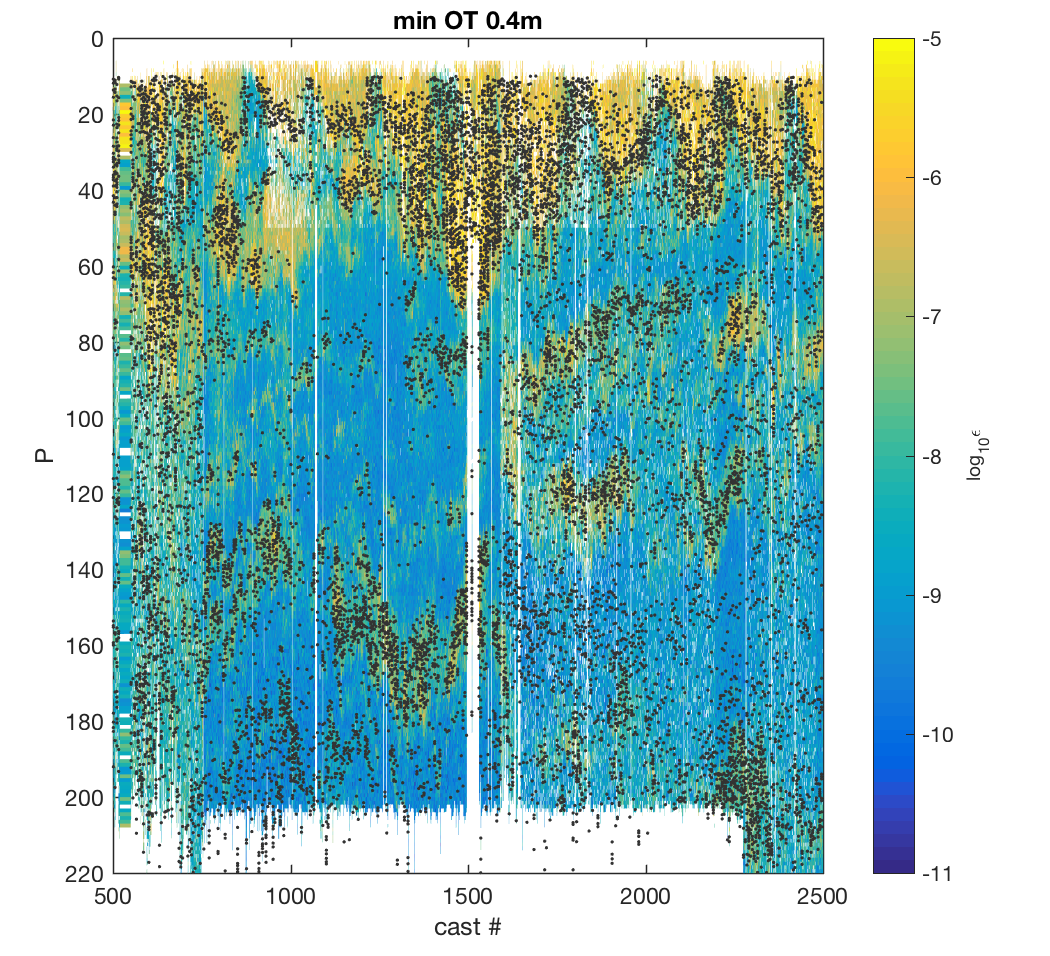
\includegraphics[scale=0.8]{eq14_minOT_40_usetemp_1_patch_locs.png}
\caption{Patch locations (mean depth) plotted on top of epsilon.}
\label{}
\end{figure}


% gamma for all binned data
\begin{figure}[htbp]
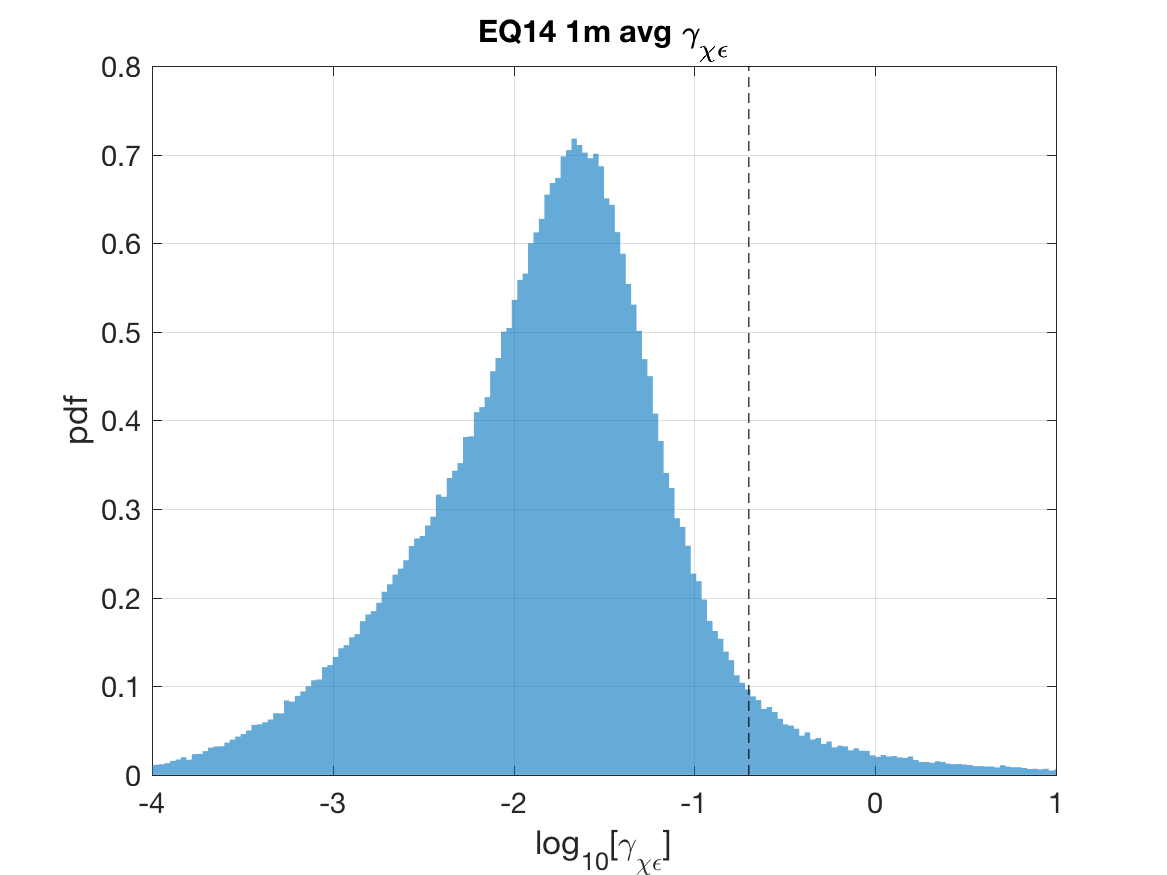
\includegraphics[scale=0.8]{eq14_binned_gamma.png}
\caption{Histogram of $\gamma_{\chi\epsilon}$ for 1m avg chameleon profiles between 60-200m depth. Vertical dashed line shows $\gamma=0.2$.}
\label{avggam}
\end{figure}

% gamma for just patches
\begin{figure}[htbp]
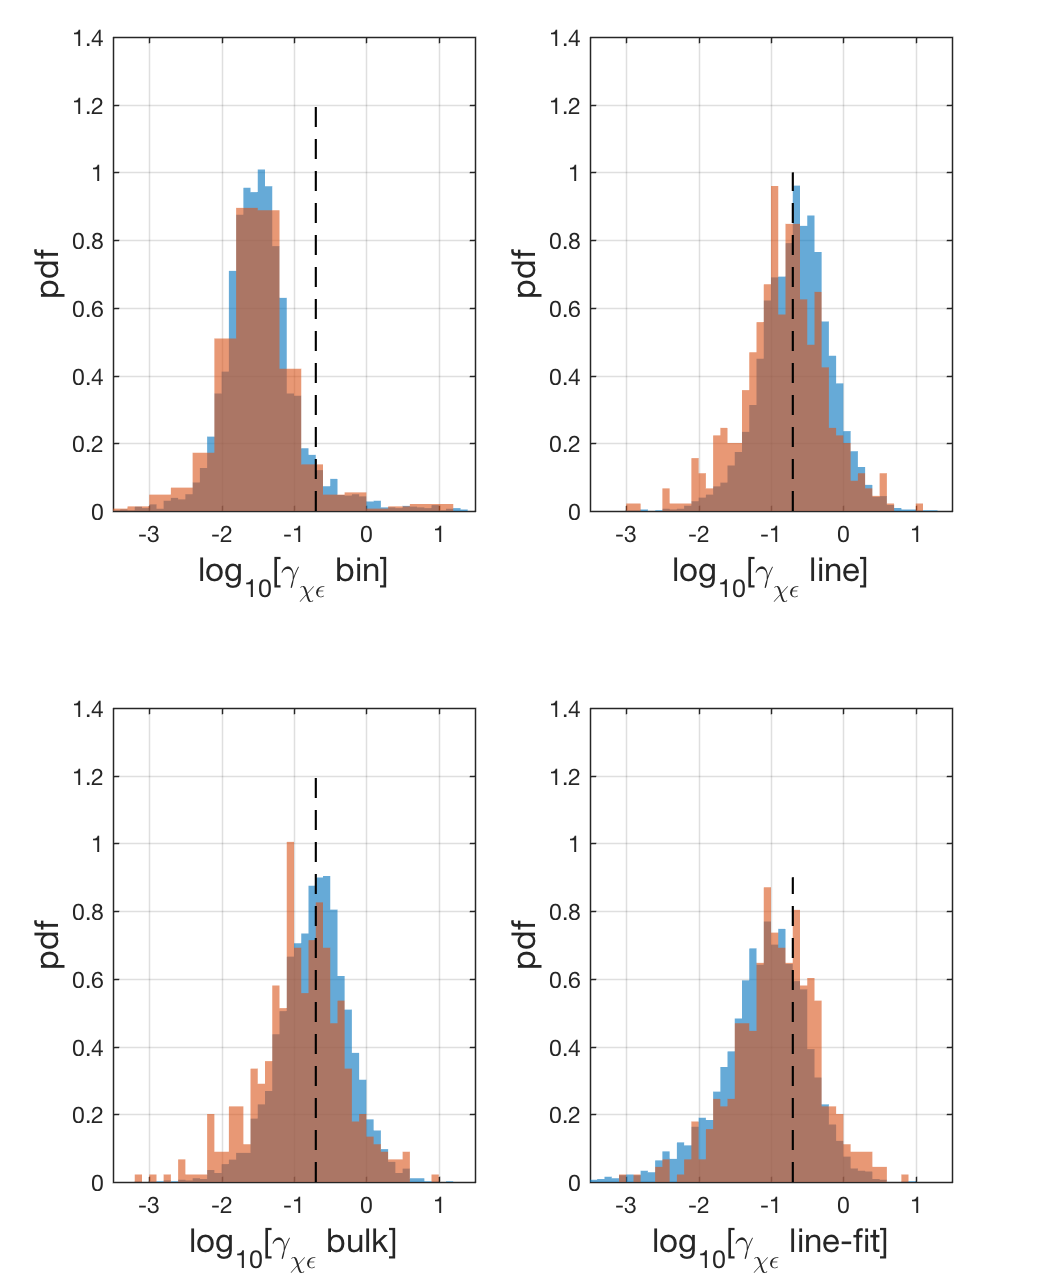
\includegraphics[scale=0.8]{eq14_minOT_40_usetemp_1_gammas_hist2X2_depth_80_200m.png}
\caption{Histogram of $\gamma_{\chi\epsilon}$ for patches, using different estimates of $N^2$ and $T_z$. Vertical dashed line shows $\gamma=0.2$. For all profiles, all depths.}
\label{patchgam}
\end{figure}

%\begin{figure}[htbp]
%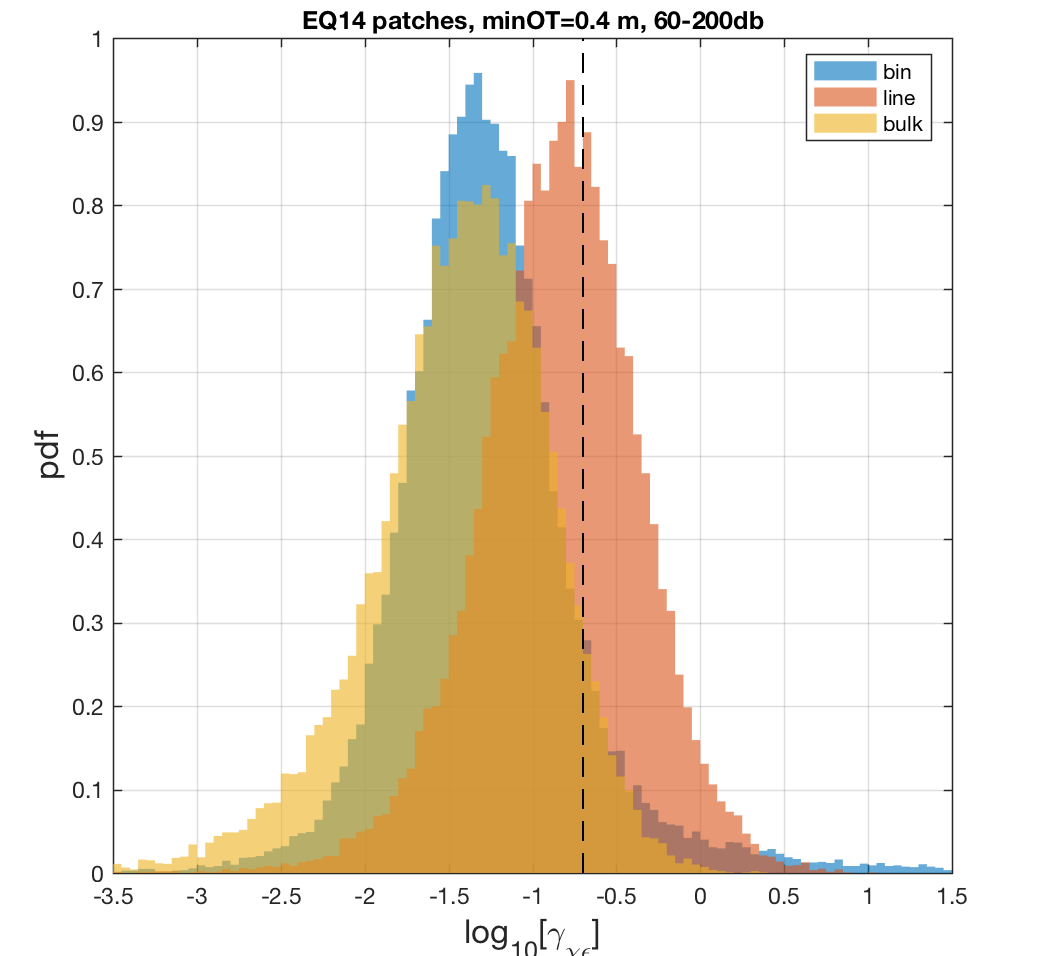
\includegraphics[scale=0.8]{eq14_minOT_40_usetemp_1_gammas_hist_cast_1_3100_zrange_60_200.png}
%\caption{Histogram of $\gamma_{\chi\epsilon}$ for patches, using different estimates of $N^2$ and $T_z$. Vertical dashed line shows $\gamma=0.2$. For all profiles, depths 60-200m only.}
%\label{patchgam}
%\end{figure}

\clearpage
%~~~~~~~~~~~
\subsection{Using smaller fmax?}

I believe the Chameleon data processed by Sally used the standard fmax=32Hz correction/cutoff for the thermistor data. However when I was trying to apply the $\chi$pod method to that data, I looked at some spectra and it looked like the thermistor rolled off much lower, around maybe 7-10hz. So I re-ran the processing using fmax=7hz. Estimates of $\gamma_{\chi\epsilon}$ are about 2-3 times larger (Figure \ref{avggam7hz}), but still significantly less than 0.2 .

% plot of binned gamma using fmax=7?
% gamma for all binned data
\begin{figure}[htbp]
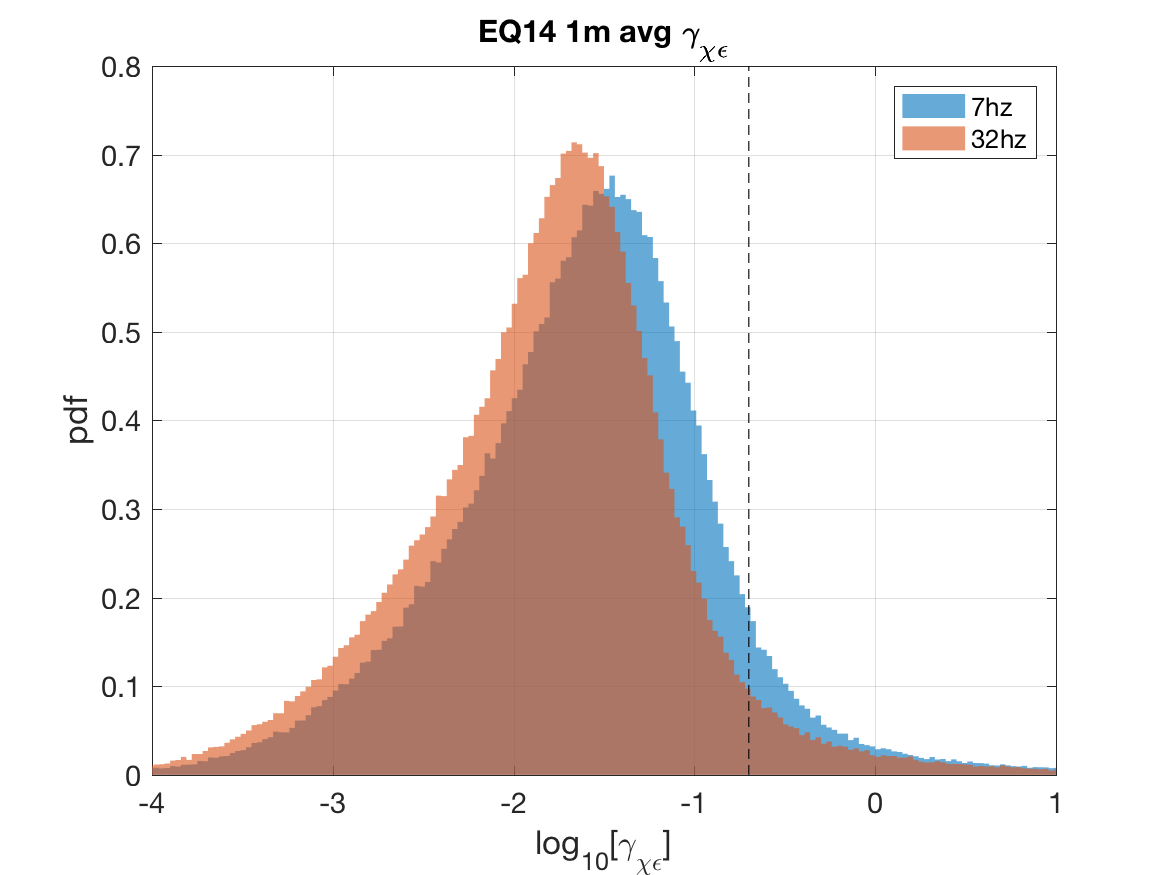
\includegraphics[scale=0.8]{eq14_binned_gamma_7hz.png}
\caption{Histogram of $\gamma_{\chi\epsilon}$ for 1m avg chameleon profiles, for standard fmax32hz as well as fmax7hz. Vertical dashed line shows $\gamma=0.2$.}
\label{avggam7hz}
\end{figure}


\clearpage
%~~~~~~~~~~~~~~~~
\subsection{Variation of $\gamma_{\chi\epsilon}$ with epsilon}

See Figure \ref{epsvsgam}:
\begin{itemize}
\item For `bin' and `linefit' methods, $\gamma$ does not show much dependence on $\epsilon$. But magnitude is less than 0.2 .
\item For `line' and `bulk' methods, magnitude of $\gamma$ is closer to 0.2, but shows an inverse dependence on $\epsilon$.
\end{itemize}


\begin{figure}[htbp]
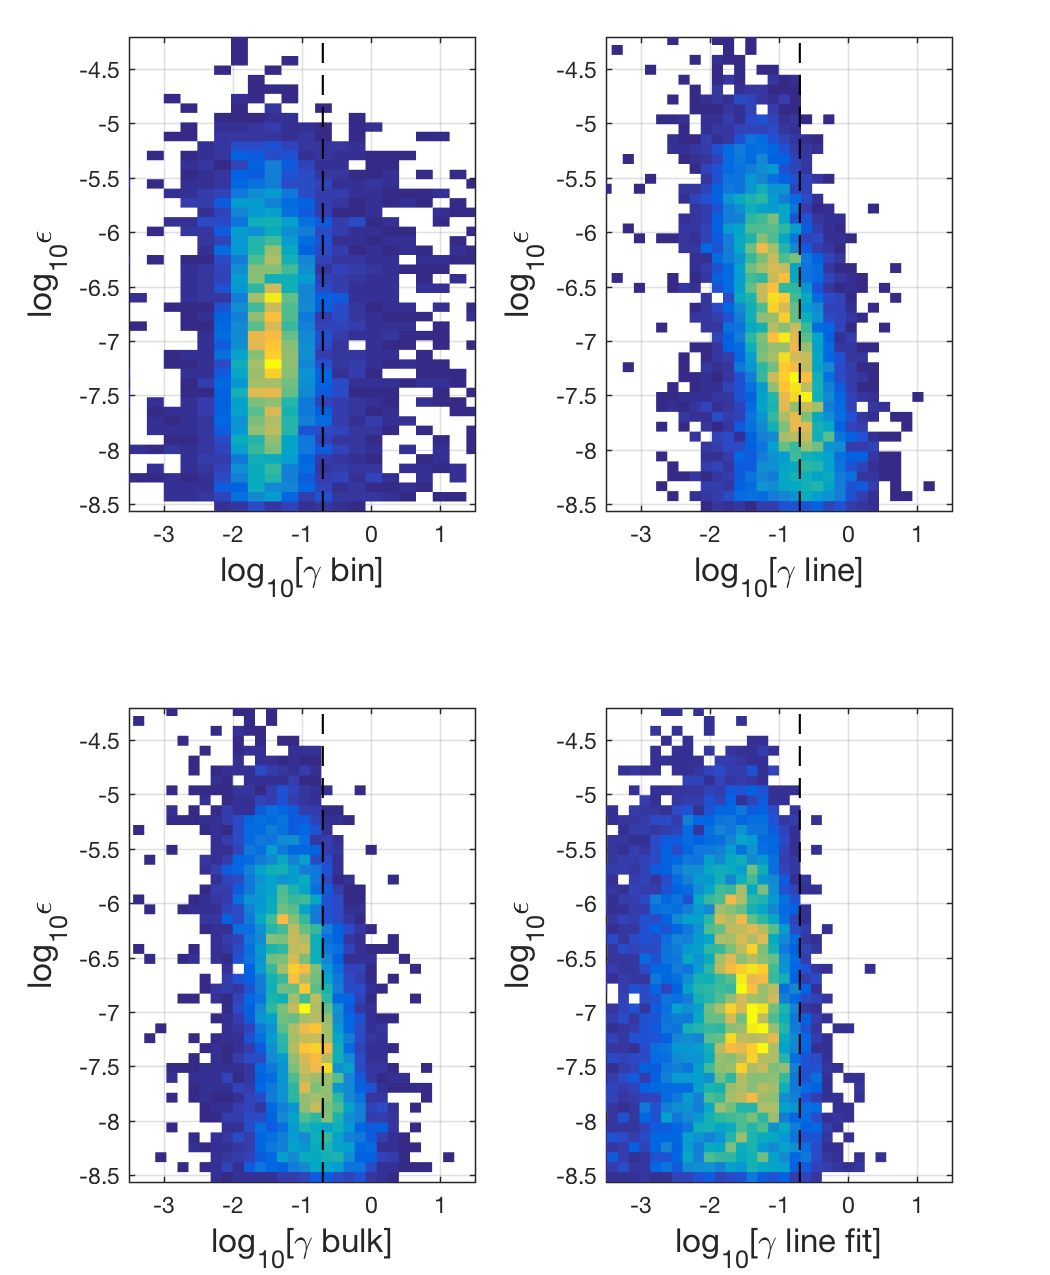
\includegraphics[scale=0.8]{eq14_minOT_40_usetemp_1_gammas_vs_eps2X2.png}
\caption{Plot of $\epsilon$  versus $\gamma_{\chi\epsilon}$ for patches.  Vertical line is $\gamma=0.2$.}
\label{epsvsgam}
\end{figure}




\clearpage
%~~~~~~~~~~~~~~~~
\subsection{Variation of $\gamma_{\chi\epsilon}$ over time}

To investigate whether $\gamma_{\chi\epsilon}$ varies over time, I plotted $\gamma_{\chi\epsilon}$ vs cast number (Figure \ref{gamvscnum}).

\begin{figure}[htbp]
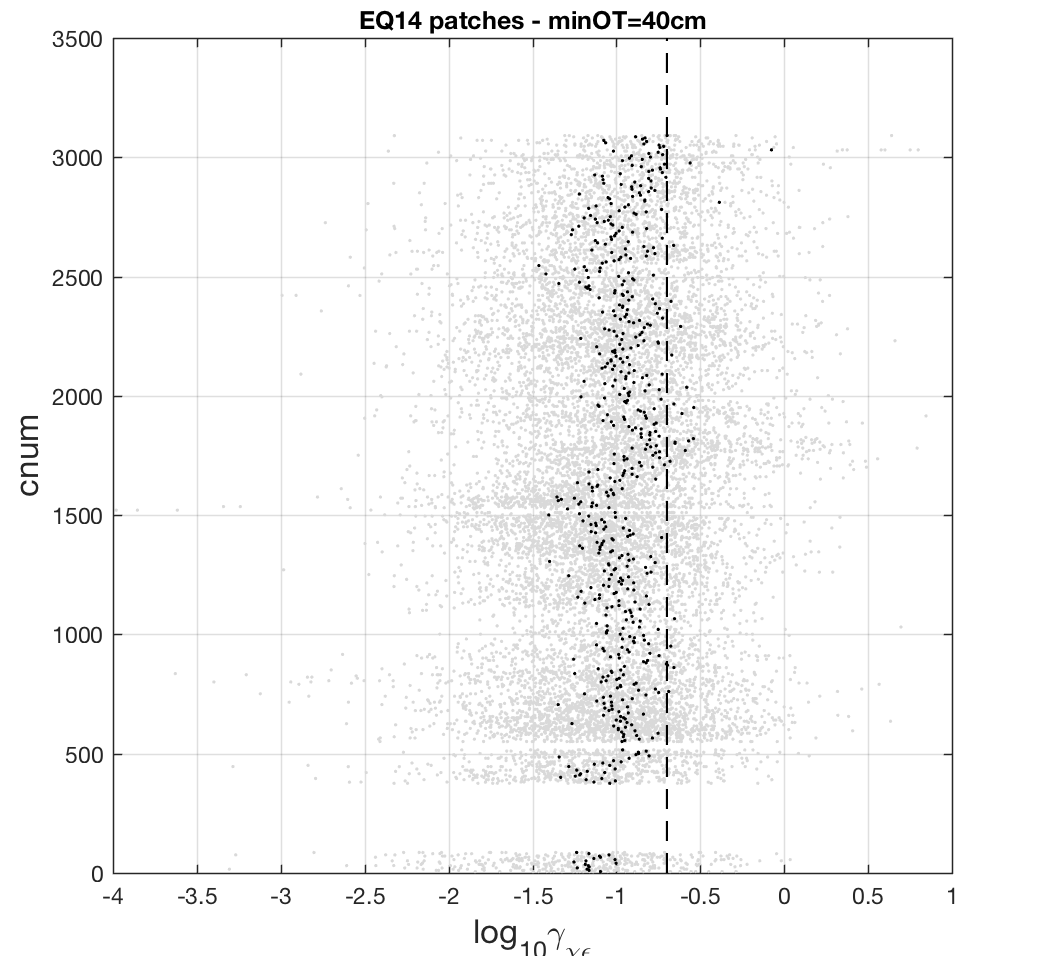
\includegraphics[scale=0.8]{eq14_minOT_40_usetemp_1_gam_vs_cnum.png}
\caption{Plot of $\gamma_{\chi\epsilon}$ for patches vs cast number. Vertical line is $\gamma=0.2$. Black points are the median value for each cast.}
\label{gamvscnum}
\end{figure}




\clearpage
%~~~~~~~~~~~~~~~~
\subsection{Variation of $\gamma_{\chi\epsilon}$ over depth}

\begin{figure}[htbp]
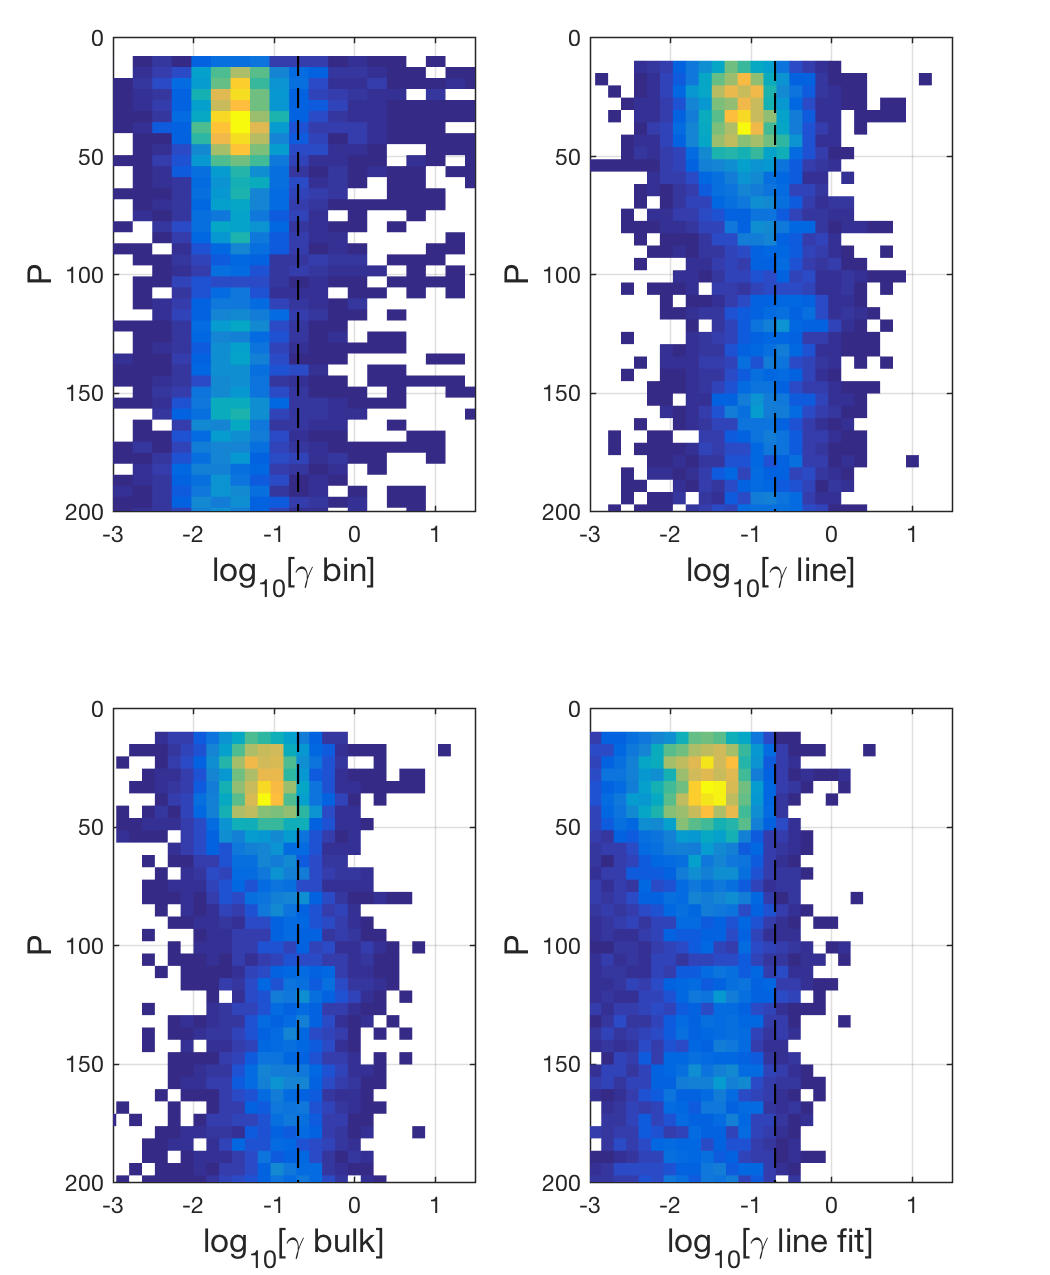
\includegraphics[scale=0.8]{eq14_minOT_40_usetemp_1_gammas_vs_depth2X2.png}
\caption{Plot of $\gamma_{\chi\epsilon}$ for patches vs depth. Vertical line is $\gamma=0.2$. }
\label{gamvsdepth}
\end{figure}





\clearpage
%~~~~~~~~~~~~~~~~~~~~~~~~~~~~~~~~~~~~~~~~
\section{Application of $\chi$pod method to patches}

The $\chi$pod method was applied to patches to see if the agreement between $\chi$pod-estimated $\chi$ and $\epsilon$ improved. Applying the $\chi$pod method to the entire profiles gave decent agreement in $\chi$, but $\chi$pod-estimated $\gamma$ was biased low by about an order of magnitude (which is what motivated this whole patch analysis).  The $\chi$pod method is applied in \verb+ComputeChi_Chameleon_Eq14_PATCHES.m+, using $N^2$ and $T_z$ from patches. It was done using both the actual $\gamma$ from patches to test, and a constant $\gamma=0.2$. All the profiles are combined into one structure in \verb+Combine_ChipodMethodPatches.m+.

\begin{itemize}
\item The magnitudes of $\chi$pod estimated $\epsilon$ for patches are closer to the actual chameleon values when using patch vs binned data (Figure \ref{epscomp2d},lower panels). However, the slope appears to be less than one for the patch estimates (lower right panel).
\item The ratio of $\chi$pod estimated $\epsilon$ to chameleon $\epsilon$ (Figure \ref{epscomphist}) is improved when using patches instead of binned data. 
\item ** checking if bulk vs line makes a difference **
\end{itemize}


\begin{figure}[htbp]
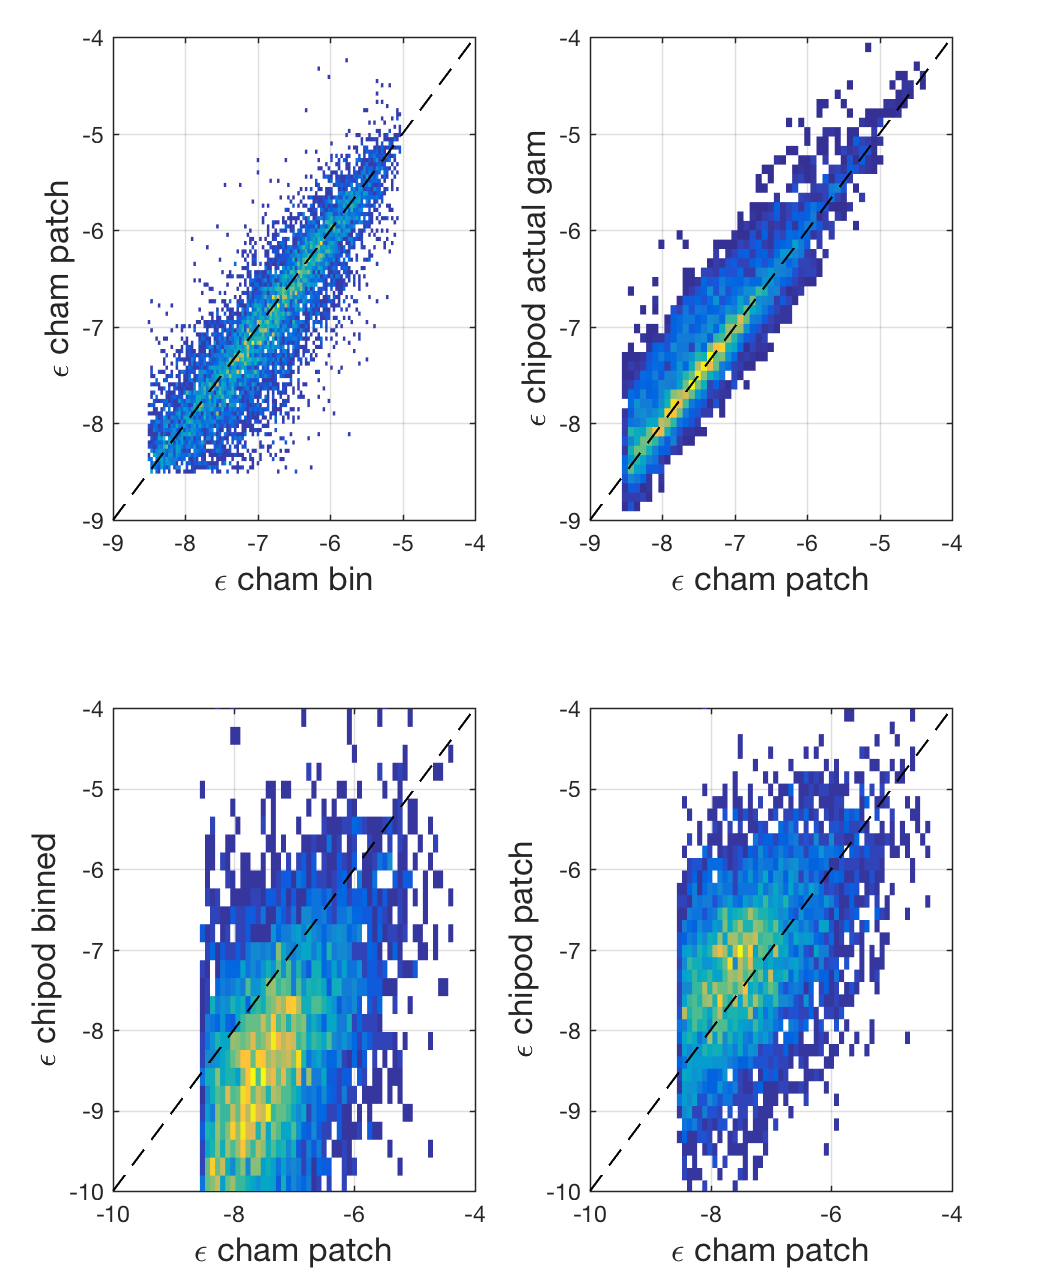
\includegraphics[scale=0.8]{ChiPatchEpsCompare_N2dTdz_line_minOT40_usetemp_1.png}
\caption{Comparison of $\epsilon$ from chameleon and $\chi$pod method applied to patches. (Top-left) Comparison of $\epsilon$ from patches to binned $\epsilon$ interpolated to patch locations. (Top-right) $\epsilon$ from $\chi$pod method using actual patch $\gamma$ to patch $\epsilon$ from chameleon. (Lower-left) $\epsilon$ from $\chi$pod method using binned data, interopolated to patch locations, compared to patch $\epsilon$ from chameleon. (Lower-right) $\epsilon$ from $\chi$pod method using a constant $\gamma=0.2$ to patch $\epsilon$ from chameleon.}
\label{epscomp2d}
\end{figure}


% histogram of chipod eps to cham eps
\begin{figure}[htbp]
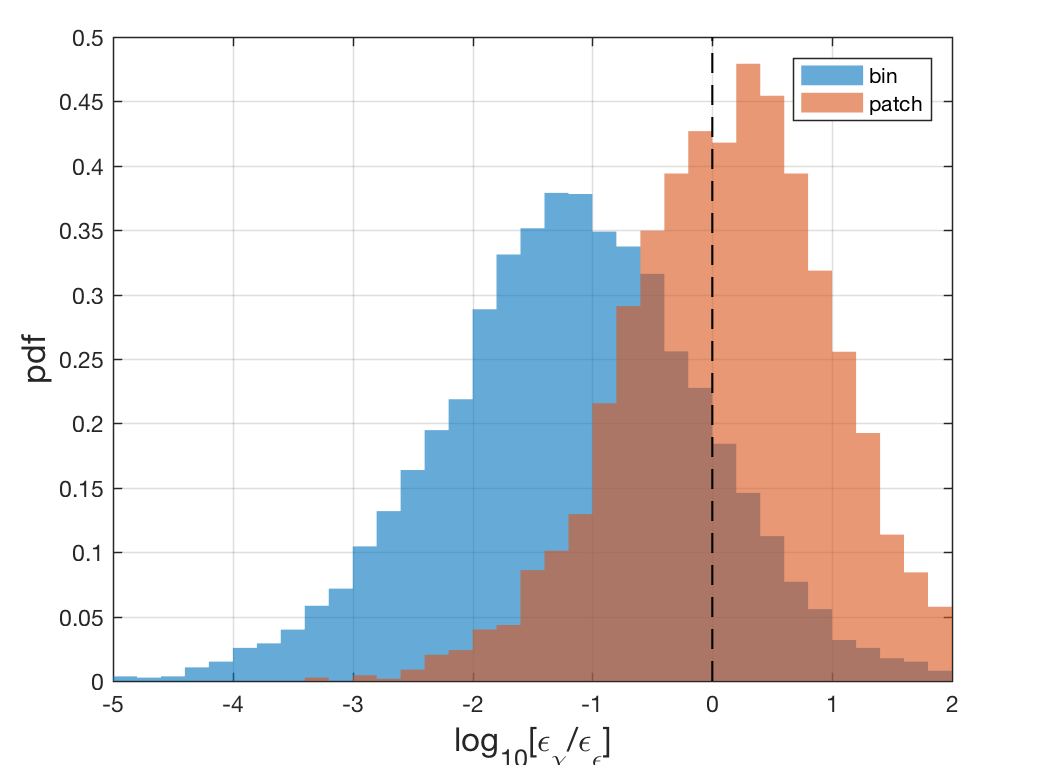
\includegraphics[scale=0.8]{ChiPatchEpsHist_N2dTdz_line_minOT40_usetemp_1.png}
\caption{Histogram of $log_{10}$ of the ratio of $\chi$pod estimated $\epsilon$ to chameleon $\epsilon$ for patches, for both binned data (interpolated to patch locations), and using only patch data.}
\label{epscomphist}
\end{figure}





\clearpage
%~~~~~~~~~~~~~~~~~~~~~~~~~~~~~~~~~~~~~~~~
\section{Summary}

\begin{itemize}
\item $\gamma_{\chi\epsilon}$ computed from 1m binned data (the standard Chameleon processing) is about 10 times smaller than the typical assumed value of 0.2.
\item $\gamma_{\chi\epsilon}$ computed for just patches varies depending on what method of choosing $T_z$ and $N^2$ is used. The `line' and `bulk' methods give $\gamma$ estimates close to 0.1. 
\end{itemize}



\end{document}  


